\documentclass{beamer}

\usepackage[english]{babel}
\usepackage{multirow}
\usepackage{amsmath,amsthm}
\usepackage{amsfonts}
\usepackage{xkeyval}
\usepackage{graphics}
\usepackage{url}
\usepackage[lined,boxed,linesnumbered]{algorithm2e}
\usepackage{CJKutf8} %支持中文

\mode<presentation>
{
  %\usetheme{}
  %\usecolortheme{beaver}
  % 可供选择的主题参见 beameruserguide.pdf, 第 134 页起
  % 无导航条的主题: Bergen, Boadilla, Madrid, Pittsburgh, Rochester;
  % 有树形导航条的主题: Antibes, JuanLesPins, Montpellier;
  % 有目录竖条的主题: Berkeley, PaloAlto, Goettingen, Marburg, Hannover;
  % 有圆点导航条的主题: Berlin, Dresden, Darmstadt, Frankfurt, Singapore, Szeged;
  % 有节与小节导航条的主题: Copenhagen, Luebeck, Malmos, Warsaw
  %\setbeamercovered{transparent}
  % 如果取消上一行的注解 %, 就会使得被覆盖部分变得透明(依稀可见)
}
\definecolor{kured}{RGB}{0,128,0}
\definecolor{kuredlys}{RGB}{34,139,34}
\definecolor{kuredlyslys}{RGB}{46,139,87}
\definecolor{kuredlyslyslys}{RGB}{60,179,113}
\setbeamercovered{transparent} %设置半透明化尚未出现的内容
\mode<presentation>
{
  \usetheme{Antibes}
  \usecolortheme[named=kured]{structure}
  \useinnertheme{circles}
  \usefonttheme[onlymath]{serif}
  \setbeamercovered{transparent}
  \setbeamertemplate{blocks}[rounded][shadow=true]
}


\logo{
\includegraphics[scale=0.08]{images/HUSTLogo}}%Logo of the presentation
\title{Multimodal semi-supervised learning for image classification}
\subtitle{M Guillaumin,J Verbeek,C Schmid-CVPR2010}
\author{Yunfei Wang}
\institute{Department of Computer Science \& Technology \\ Huazhong University of Science \& Technology}
\date{\today}

\begin{document}

\begin{CJK*}{UTF8}{gbsn} %中文支持

\begin{frame}
\titlepage
\end{frame}


\begin{frame}\frametitle{Table of contents}
\tableofcontents
\end{frame}

\section{Introduction}
\begin{frame}\frametitle{Motivation}
\begin{itemize}
\item Increasing quantity and diversity of hand-labelled images improves the performance of classifier.
\item Labelling images is time consuming and unrealistic in some scenario.
\item \textcolor{blue}{Motivation:Using other information sources to aid learning process on limited amount of labelled images.}
\end{itemize}
\end{frame}

\section{Multimodal Semi-supervised Learning}
\subsection{Supervised Learning}
\begin{frame}[allowframebreaks]\frametitle{Supervised Learning}
Train a SVM on labelled images:
\begin{equation}
f(x)=\sum_i\alpha_ik(x,x_i)+b
\end{equation}
where $k(\cdot,\cdot)$ is kernel function.\\
Class label:
\[
y\in\{-1,+1\}=sign(f(x))
\]
\end{frame}

\begin{frame}\frametitle{Combine visual and textual representations}
Combined kernel:
\begin{equation}
k_c(\cdot,\cdot)=d_vk_v(\cdot,\cdot)+d_tk_t(\cdot,\cdot)
\end{equation}
where $k_v(\cdot,\cdot)$ is visual kernel,$k_t(\cdot,\cdot)$ is textual kernel,$d_v,d_t>0$ and $d_v+d_t=1$.\\

\textcolor{red}{Multiple kernel learning(MKL) framework} allows joint learning of kernel combination weights $d_v$,$d_t$ and the parameters $\{\alpha_i\}$ and $b$.
\textcolor{blue}{The SVM based on combined kernels:}
\begin{equation}
f_c(x)=\sum_i\alpha_ik_c(x,x_i)+b
\end{equation}
\end{frame}

\subsection{Semi-supervised Learning}
\begin{frame}[allowframebreaks]\frametitle{Semi-supervised Learning}
Notation:$\mathcal{L}$ is set of labelled images;$\mathcal{U}$ is set of unlabelled images.\\
\begin{block}{Processing tactics}
\begin{enumerate}
\item Learn a joint visual-textual classifier $f_c$form $\mathcal{L}$ using MKL;
\item Predict class labels for images in $\mathcal{U}$ with $f_c$;
\item Train a visual-only SVM classifier $f_v$ from $\mathcal{L}$ and $\mathcal{U}$;
\item Complete image classification task with $f_v$.
\end{enumerate}
\end{block}
\end{frame}

\subsection{Alternative approachs}
\begin{frame}\frametitle{First Alternative}
\textcolor{red}{Intention}:Only add the confidently classified examples in $\mathcal{U}$,those fall outside the margin with $|f_c(x)|\geq 1$.\\
\begin{center}
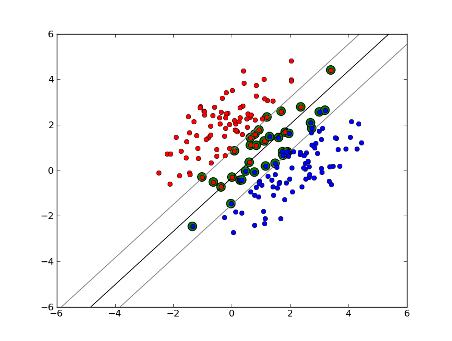
\includegraphics[scale=0.4]{images/svm_soft}
\end{center}
They have the less possibility of changing the MKL classifier.
\end{frame}

\begin{frame}\frametitle{Second Alternative}
\textcolor{red}{Intention}:Approximate the joint classification function $f_c$.\\
Perform a least square regression(LSR) on MKL scores $f_c(x)$ for all examples in $x\in\mathcal{L}\cup\mathcal{U}$ to find the function 
\[
f_v(x)=\sum_i\alpha_ik_v(x,x_i)+b
\]
\end{frame}

\begin{frame}\frametitle{Pseudo-code of the algorithm}
\begin{center}
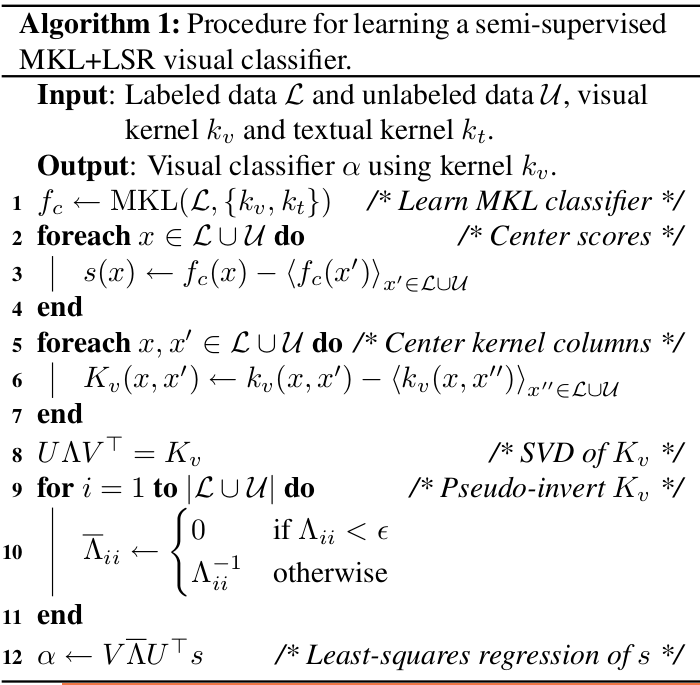
\includegraphics[scale=0.3]{images/algorithm}
\end{center}
\end{frame}

\end{CJK*}
\end{document}
